\chapter{Experimente}\label{chap:experiments}

Nach der Beschreibung des Konzept und Verlauf des Python-Skripts geht dieses Kapitel auf die wichtigsten Trainingsdurchläufe ein und diskutiert die Ergebnisse. 
\\\\
Es wurden iterativ Trainingprozeduren durchgeführt mit jeweils unterschiedlichen Konfiguration, wie um vorherigen Kapitel gezeigt, und miteinander verglichen. Die genauen Konfigurationen werden bei den einzelnen Experimenten angeführt. Die Experimente liefen auf einem Rechner mit NVIDIA TITAN Xp 12 GB VRAM Grafikkarte, Intel i7-7800X CPU und 32 GB RAM. Da diese Arbeit zeitlich begrenzt ist, wurden die Experimente auf max. 100 Epochen begrenzt, was die durchschnittliche Laufzeit auf etwa drei bis vier Stunden je Experiment bringt. Diese Beschränkung wirkt ebenfalls Overfitting entgegen, da nicht ausreichend Zeit hat, um sich auf den Trainingsdatensatz "`einzugewöhnen"'.
\\\\
Es wurden drei unterschiedliche Datensätze aus den Sentinelprodukten erzeugt. 
\begin{enumerate}
	\item Der originale unaugmentierte Datensatz enthält insgesamt jeweils zwölf Bilder und Masken\footnote{Trainingsanteil: 7, Validationsanteil: 2, Testanteil: 3} und dient als Basis für das Ausgangsexperiment. 
	\item Der augmentierte Datansatz (s. Kapitel \ref{sec:augmentation}) enthält 1291 Dateien und Masken\footnote{Trainingsanteil: 825, Validationsanteil: 207, Testanteil: 259}. Nachdem die zufällige Ausschnitte produziert wurden, kam es vor, dass einige Masken keinen \textit{RoI}-Anteil enthielten. Diese Masken und auch die zugehörigen Bilddateien wurden verworfen und weicht deswegen von der eigentlichen Größe von 1296 Elementen\footnote{Die zwölf ursprünglichen Dateien multipliziert mit dem Data Augmentation-Faktor von 108.} ab.
	\item In einem dritten Datensatz wurden Ausschnitte benutzt, deren Bildgrenzen sich an den äußersten Punkten der Masken befinden (s. Abb. \ref{fig:example-overfitting}). Dieser Datensatz wurde ausschließlich mittels Rotationen erweitert und enthält 144 Elemente\footnote{Trainingsanteil: 92, Validationsanteil: 23, Testanteil: 29}. 
\end{enumerate}
\noindent

\subsubsection{Experimente 1}\label{sub:sub:sec:experiment-1}

\begin{lstlisting}[language=python,caption={Konfiguration für Experimente 1},captionpos=b]
class CropDiseaseConfig(Config):
    BACKBONE = "resnet50"
    IMAGE_MAX_DIM = 128
    IMAGE_MIN_DIM = 128
    IMAGE_RESIZE_MODE = "square"
    IMAGES_PER_GPU = 4
    LEARNING_RATE = 0.001
    NUM_CLASSES = 1 + 1
    RPN_ANCHOR_SCALES = (8, 16, 32, 64, 128)
    STEPS_PER_EPOCH = 3
    USE_MINI_MASK = False
\end{lstlisting}
\noindent
Zuerst wurden ein Modell auf Datensatz 1 und alle Schichten des Modells wurden trainiert. Diese Experimente sollen zeigen, wie ein zu kleiner Datensatz sich auswirken kann.

\begin{figure}[ht]
	\centering
    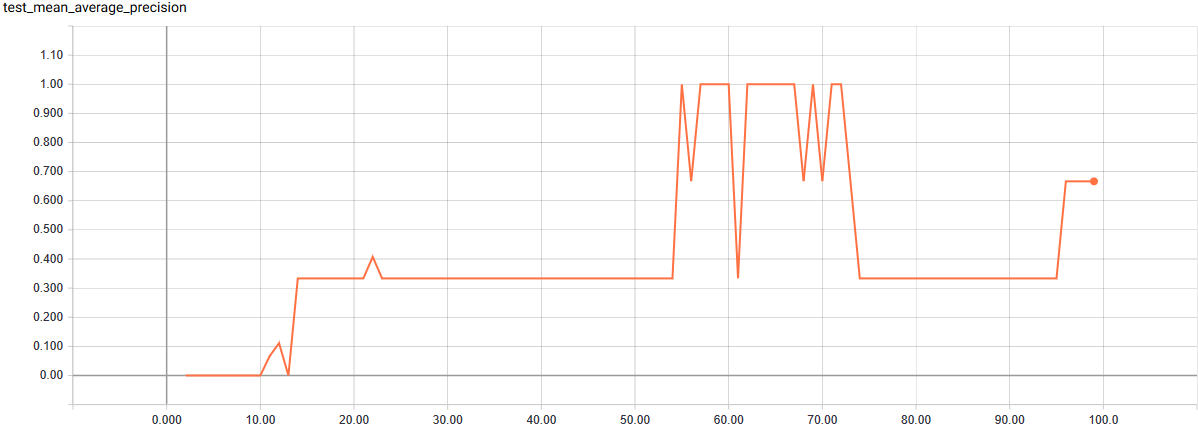
\includegraphics[width=.7\textwidth]{pics/map-1.PNG}
    \caption{\textit{mAP}-Graph von Experiment 1, X-Achse: Epochennummer, Y-Achse: \textit{mAP}-Werte}
    \label{fig:map-1}
\end{figure}
\begin{figure}[ht]
	\centering
    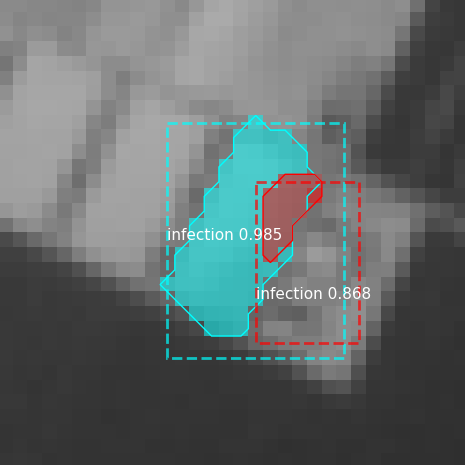
\includegraphics[height=3.5cm]{pics/pred-1-1.png}
    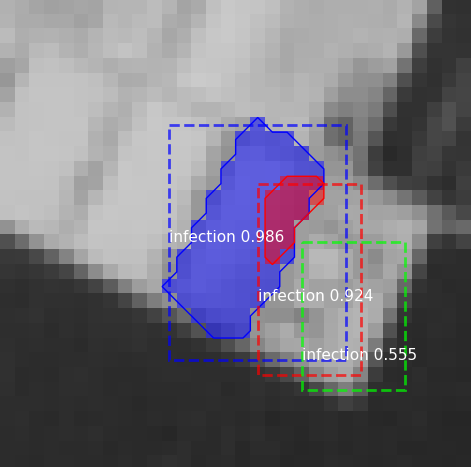
\includegraphics[height=3.5cm]{pics/pred-1-2.png}
    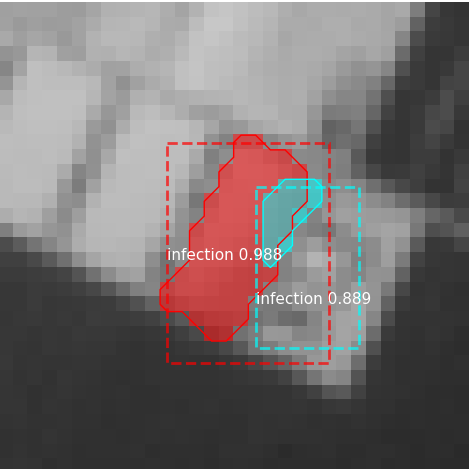
\includegraphics[height=3.5cm]{pics/pred-1-3.png}
    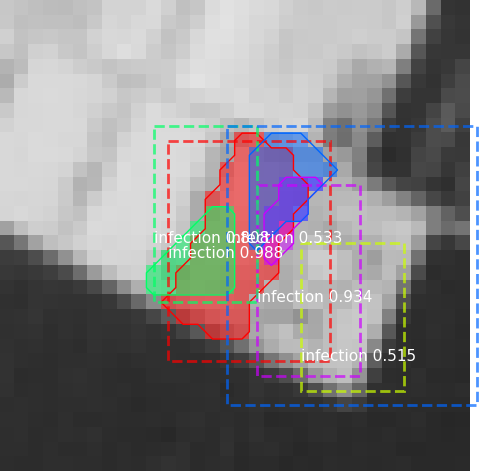
\includegraphics[height=3.5cm]{pics/pred-1-4.png}
    \caption[Beispielvorhersagen Experiment 1]{Beispielvorhersagen anhand der Gewichte von Epoche 55}
    \label{fig:pred-1}
\end{figure}
\noindent
Man sieht, dass das Modell während des Trainings unterdurchschnittliche Ergebnisse erzielt, was wenig überraschend ist, da der Datensatz sehr klein ist. Da nach jeder Epoche die Gewichte zwischengespeichert werden, können diese einzeln geladen werden. So wurde für eine Detektion ein Modell mit den Gewichten der 55. Epoche initialisiert, da sich hier der \textit{mAP}-Wert auf dem Maximalwert befindet. Die Bilder in Abb. \ref{fig:pred-1} entstammen einem fremden Datensatz, ähneln aber in den Grundcharakteristika dem eigentlichen Datensatz 1. Zum Beispiel ist das Zielfeld ähnlich ausgerichtet und zentriert. Man sieht, dass sich die berechneten Masken relativ genau auf das Zielfeld eingrenzen. Jedoch sind die erzeugten Bounding-Boxen und passen nicht zu den entsprechenden Masken, falls eine Maske erkannt wurde. Auch wurden mehrere Objektinstanzen erkannt, wobei eine einzige Instanz detektiert werden sollte. Werden die Bilder in Abb. \ref{fig:pred-1} nun vertikal gespiegelt und in das Netzwerk gegeben, erzeugt das Modell keine Masken, obwohl lediglich die Ausrichtung verändert wurde. Das ist ein Hinweis auf Overfitting, da das neuronale Netz minimale Änderungen nicht mehr erkennt.

\subsubsection{Experimente 2}\label{sub:sub:sec:experiment-2}

\begin{lstlisting}[language=python,caption={Konfiguration für Experimente 2},captionpos=b]
class CropDiseaseConfig(Config):
    BACKBONE = "resnet50"
    IMAGE_MAX_DIM = 128
    IMAGE_MIN_DIM = 128
    IMAGE_RESIZE_MODE = "square"
    IMAGES_PER_GPU = 4
    LEARNING_RATE = 0.001
    NUM_CLASSES = 1 + 1
    RPN_ANCHOR_SCALES = (8, 16, 32, 64, 128)
    STEPS_PER_EPOCH = 3
    USE_MINI_MASK = False
\end{lstlisting}
\noindent
Bei diesem Experiment wurde ein Modell Datensatz 2 und alle Schichten des Modells trainiert. Die Konfiguration bleibt unverändert, jedoch ist hier der augementierte Datensatz vergleichweise größer.

\begin{figure}[ht]
	\centering
    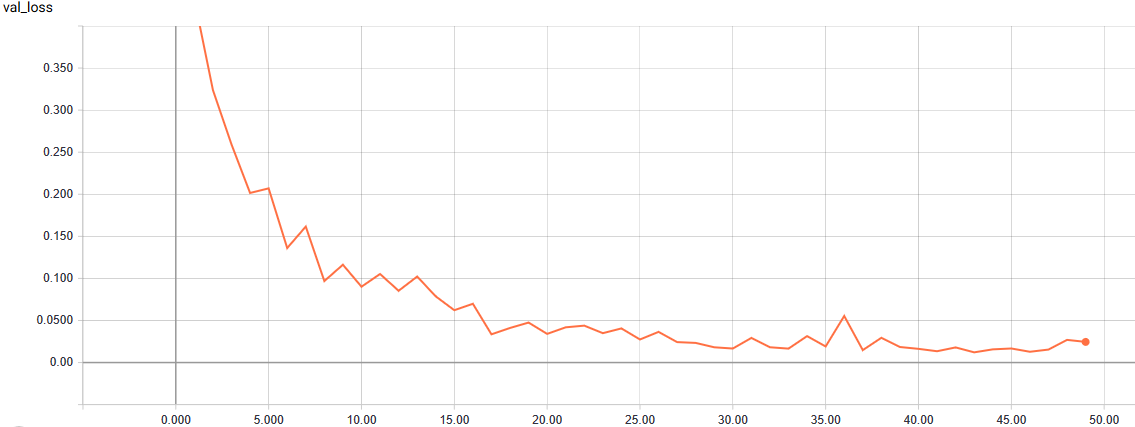
\includegraphics[width=.7\textwidth]{pics/val-loss-2.PNG}
    \caption{\textit{loss}-Graph von Experiment 2, X-Achse: Epochennummer, Y-Achse: \textit{loss}-Werte}
    \label{fig:map-2}
\end{figure}

\begin{figure}[ht]
	\centering
    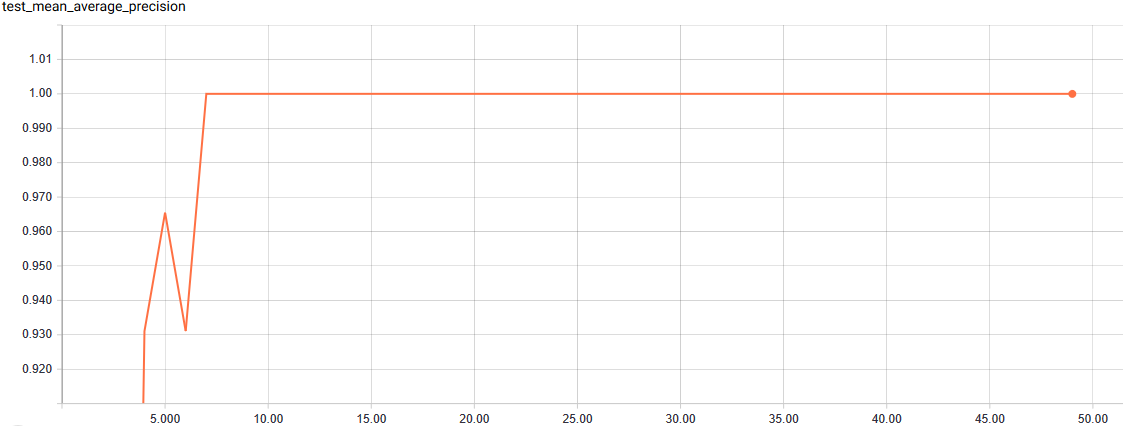
\includegraphics[width=.7\textwidth]{pics/map-2.PNG}
    \caption{\textit{mAP}-Graph von Experiment 2, X-Achse: Epochennummer, Y-Achse: \textit{mAP}-Werte}
    \label{fig:map-2}
\end{figure}

\begin{figure}[ht]
  \centering
  \begin{minipage}[c]{.3\textwidth}
  \centering
  
\includegraphics[height=2cm]{pics/roi-2-1.png}
  \\ \vspace{.5cm}
  
\includegraphics[height=3cm]{pics/roi-2-2.png}
  \\ \vspace{.5cm}
  
\includegraphics[height=3cm]{pics/roi-2-3.png}
  \end{minipage}
  \begin{minipage}[c]{.3\textwidth}
  \centering
  
\includegraphics[height=2cm]{pics/mask-2-1.png}
  \\ \vspace{.5cm}
  
\includegraphics[height=3cm]{pics/mask-2-2.png}
  \\ \vspace{.5cm}
  
\includegraphics[height=3cm]{pics/mask-2-3.png}
  \end{minipage}
  \begin{minipage}[c]{.3\textwidth}
  \centering
  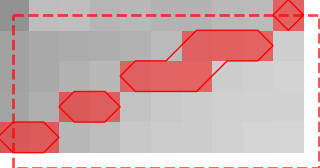
\includegraphics[height=2cm]{pics/pred-2-1.png}
  \\ \vspace{.5cm}
  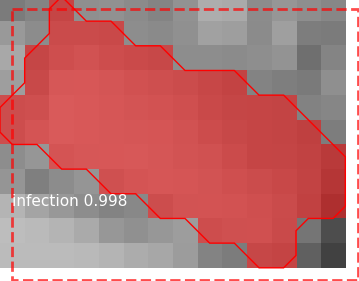
\includegraphics[height=3cm]{pics/pred-2-2.png}
  \\ \vspace{.5cm}
  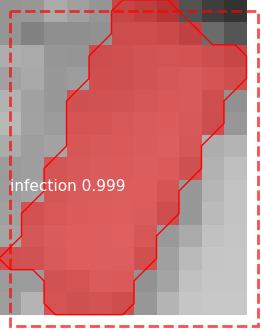
\includegraphics[height=3cm]{pics/pred-2-3.png}
  \end{minipage}

  \caption[Beispielvorhersagen Experiment 2]{Beispielvorhersagen anhand der Gewichte von Epoche 37}
  \label{fig:example-overfitting}
\end{figure}

Die \textit{mAP}-Kurve konvergiert ab Epoche 7 gegen $1$ und verweilt dort. Dagegen sinken die $loss$-Werte weiterhin